% NESSF 2014 proposal

\documentclass[12pt]{article}

%% Use pdfTex to insure the margin sizes in Windows

\usepackage{natbib}
%\usepackage{natbib,natbibspacing}
\setlength{\bibsep}{3pt} % spacing for bibliography items
\citestyle{aa} % apj type
%\citestyle{plain} ; number style

% try smaller section title fonts
\usepackage{sectsty}
\sectionfont{\large}
\subsectionfont{\normalsize}

\pdfpagewidth=8.5in
\pdfpageheight=11in

\setlength\topmargin{-0in}
\setlength\headheight{0in}
\setlength\headsep{0in}
\setlength\textheight{9in}
\setlength\textwidth{6.5in}
\setlength\oddsidemargin{0in}
\setlength\evensidemargin{0in}

\usepackage{mathrsfs}
\usepackage{amsmath,amssymb}
\usepackage{verbatim}
\usepackage{wrapfig}

\usepackage{enumitem}

% journal names
\usepackage{aas_macros}

\newcommand{\beq}{\begin{equation}}
\newcommand{\eeq}{\end{equation}}
\def\etal{~et~al.~}
%\def\mps{m~s$^{-1}$}
\def\mps{m/s}
\def\msini{M\sin{i}}
\def\mjup{M_{\rm Jup}}
\def\msol{M_{\odot}}
\def\mearth{M_{\oplus}}
\def\degree{^{\circ}}
\def\leq{\leqslant}
\def\geq{\geqslant}
\def\kepler{{\it Kepler}}
\def\minerva{{\it Minerva}}
\def\hrs{HET/HRS}
\def\keck{Keck/HIRES}

\usepackage{graphicx}
%\usepackage[pdftex,bookmarks, % add hyperlinks
%colorlinks,
%plainpages=false]{hyperref}

\begin{document}

%\tableofcontents
%\newpage

%%%%%%%%%%%%%%%%%%%%%%%%%%%%%%%%%%%%%%%%%%%%%%%%%%%%%%%%%%%%%%%%%%%%%%%%%%%%%%%%%%%%%%%%%
% title
\title{\vspace{-45pt} \bf \Large Finding the Lowest Mass Exoplanets with
  \\ Improved Radial Velocimetry \vspace{-6pt}}
\author{\normalsize Sharon Xuesong Wang}
\date{}
\maketitle

%%%%%%%%%%%%%%%%%%%%%%%%%%%%%%%%%%%%%%%%%%%%%%%%%%%%%%%%%%%%%%%%%%%%%%%%%%%%%%%%%%%%%%%%%
\vspace{-30pt}
\section{Overview}

% An overview of awesomeness of finding low-mass exoplanets.
The excellent synergy between NASA's \kepler\ mission and the
ground-based radial velocity (RV) surveys has made numerous
ground-breaking discoveries of exoplanets, including many interesting
low-mass and rocky planets
\citep[e.g.,][]{howard2013,pepe2013,marcy2014}. This has brought the
field of exoplanets into an exciting era with an inceasing sample of
small and potentially rocky planets \citep{weiss2013} with the great
promise towards the discovery of Earth analogs in the near future.
% ZZZ add number of kepler candidates with mass measurements with RV

% But... precise RV is yet to be more precise.
In the post-\kepler\ era, radial velocimetry will undoubtedly continue
to play a key role in validating \kepler\ candidates and measuring
their masses, as well as detecting exoplanets independently. However,
the current precision of radial velocimetry (0.5--1~\mps) acts as one
of the major limiting factors in detecting lower mass
exoplanets. Breaking this limit is critical for pushing the lower mass
boundary of the exoplanet ensemble. It is also an absolutely
necessary step towards finding Earth-mass ($\mearth$) exoplanets in
the habitable zone around Sun-like stars, which requires an RV
precision of $\sim$0.1 \mps.
% ZZZ add the current mass record holders 
% ZZZ doesn't feel like a very strong `but...'; add more on necessity
% of our work.

% What we propose to do
\textbf{We propose to improve the RV precision of several leading RV
  instruments through correction of systematic errors, with the aim to
  find the lowest mass exoplanet.} Improved radial velocimetry will
also enable better characterization of the current known low RV
amplitude planetary systems. Moreover, eliminating instrumental
systematic errors will help in isolating the RV signals induced by
stellar activities and promote a better understanding of the stellar
RV jitter, which is also crucial for finding lower mass exoplanets.


%%%%%%%%%%%%%%%%%%%%%%%%%%%%%%%%%%%%%%%%%%%%%%%%%%%%%%%%%%%%%%%%%%%%%%%%%%%%%%%%%%%%%%%%%
\vspace{-3pt}
\section{Expected Scientific Outcome and Impact}

% overall
Our work will directly improve the RV precision of the two leading RV
instruments on two 10-meter-class telescopes: Keck and the
Hobby-Eberly Telescope (HET). The large collecting areas of these
telescopes make them the ideal facilities for carrying out large and
deep surveys around bright or faint stars, as well as for extensive
follow-up observations on \kepler\ planet candidate systems. Our work
will also help improving the RV precision of two
instruments on smaller telescopes: CHIRON and the upcoming Project
\minerva. Designed for carrying out dedicated surveys with extremely
high RV precision, these two instruments will provide valuable high
cadence data on nearby and bright stars, which are the best targets
for planetary atmosphere characterization studies.

% Keck
\textbf{Science with \keck: } The primary instrument we work with is
the High Resolution Echelle Spectrometer (HIRES) on Keck I (current RV
precision $\sim$1~\mps). Among the RV discovered exoplanets,
\keck\ contributed to a majority of these discoveries. It also
contributed to a great number of mass measurements of confirmed
\kepler\ planets --- in particular, \textit{most} of the low mass ones
\citep[e.g.,][]{gautier2012,gilliland2013,howard2013,marcy2014}. However,
its current RV precision is limiting its ability to detect lower mass
planets or planets with the same mass but further out in orbit
\citep[e.g.,][]{marcy2014}.

% Lots of low mass Kepler planets
Our work will improve the RV precision of \keck, and thus extend the
lower mass limit of the current exoplanet sample. This is especially
promising when considering the large candidate pool that
\kepler\ provides: among the 1600 KOIs with transit signals suggesting
a planet radius smaller than 2 Earth radii ($R<2\cdot R_{\oplus}$),
there are 260 whose host stars have \kepler\ magnitude $< 13$ and are
thus bright enough for Keck to follow up (compared with fewer than 10
such targets with \kepler\ mag $< 9$ and thus accessible by HARPS-N).

% Multi-planet systems to improve with Keck
Meanwhile, better RV precision will improve the characterization of
multiple-planet systems, especially the ones that host challenging low
RV amplitude planets/candidates and with potentially very active
dynamic interactions. We plan to reanalyze the RV data and perform
dynamic analysis on such systems, including the $\upsilon$ Andromedae
system, the first multi-planet system discovered around main-sequence
star \citep{butler1999,wright2009,curiel2011}, as well as the GJ 581
system, which hosts the first claimed terrestrial-mass exoplanet in
the Habitable Zone \citep{vogt2010} though under debate
\citep[e.g.,][]{gregory2011,vogt2012,robertson2013}. 

% HET
\textbf{Science with \hrs: } We also work with another leading RV
instrument on a 10-meter-class telescope: the High Resolution
Spectrograph (HRS) on HET (current RV precision $\sim$3--5~\mps). With
multiple ongoing upgrades on \hrs\ (expected to finish in summer
2014), its throughput will be improved by a factor of $\sim$5, also
with the promise of a higher RV precision of the new HRS. HET will
become the second telescope, besides Keck, that is suitable for RV
follow-up on the stars hosting planet candidates discovered by
\kepler. This will make the \kepler\ follow-up programs more
efficient. It will also benefit other planet search programs on
\hrs\ such as surveys on long-period planets and multiple-planet
systems.

% Minerva and CHIRON
\textbf{Minerva and CHIRON: } Our work also has great synergy with two
very high RV precision instruments on smaller telescopes: the upcoming
project \minerva\ and CHIRON on
the 1.5m SMARTS telescope at CTIO. 

Project \minerva\ consists an array of four 0.7m telescopes and a
vacuum-sealed highly-stable spectrograph that will perform dedicated
RV monitoring on a carefully-selected ensemble of nearby stars. It is
expected to discover $\gtrsim 10$ Earth- to super-Earth-size planets
with orbital period of 1--100 days around nearby stars, with 3--5
expected to be in the Habitable Zones of their host stars
\citep{bottom2013,hogstrom2013}. The proposed work here will help
prepare the project to meet its targeted long-term RV precision of
$\sim 0.8$~\mps.

CHIRON has demonstrated short-term RV stability of $\sim0.5$~\mps on
$\tau$ Ceti \citep{chiron2013}. The improvement we propose will help
CHIRON achieve long-term RV stability below 1~\mps\ and help validate
or characterize the potential planetary systems in $\tau$ Ceti
\citep{tuomi2013} and $\alpha$ Centauri Bb
\citep{dumusque2012,hatzes2013}, which both have exoplanets with RV
amplitudes on the order of $\sim 1$~\mps\ or even smaller.


%---------------------------------------------------------------------------------------
% RECYCLE BIN
\begin{comment}

The field of exoplanet is progressing in a fast pace towards the
discovery of Earth-like planets around other stars. During the past
decades, we have moved on from the age of booming discoveries of
Jupiter-mass exoplanets via radial velocimetry (add ref) to the
\kepler\ era where there are thousands of Earth- and super-Earth-size
exoplanet candidates (add ref). Moreover, great promises lie ahead with
future ground-based instruments (e.g., ESPRESSO; add ref) or space
missions (e.g., TESS; add ref).

\begin{itemize}[leftmargin=2.2em]
    \vspace{-3pt}
\item Improve the RV precision of Keck through eliminating known
  systematics and improved statistics.
    \vspace{-3pt}
\end{itemize}

\end{comment}
%---------------------------------------------------------------------------------------


%%%%%%%%%%%%%%%%%%%%%%%%%%%%%%%%%%%%%%%%%%%%%%%%%%%%%%%%%%%%%%%%%%%%%%%%%%%%%%%%%%%%%%%%%
\vspace{-3pt}
\section{Methodology}

Through our pilot study, we have
identified several contributing factors to RV systematic errors,
some of which are being recoganized and studied in detail \textit{for the
very first time}. These factors contribute to the RV error budget at
$\sim$1~\mps\ level, and thus they set the floor of long-term RV
precision at 1~\mps\ if not carefully studied and corrected for.


We propose to fix the following things:
\begin{itemize}
  \item Telluric lines.
  \item Wavelength-dependent statistical weighting.
  \item Iodine FTS validation.
  \item Data reduction and IP analysis.
\end{itemize}



\begin{wrapfigure}{r}{0.51\textwidth}
  \vspace{-35pt}
  \begin{center}
    \includegraphics[width=0.48\textwidth]{fts}
  \end{center}
  \vspace{-25pt}  
  \caption{FTS compared with echelle spectrum.}
  \vspace{-8pt}  
  \label{fts}
\end{wrapfigure}

\begin{wrapfigure}{r}{0.51\textwidth}
  \vspace{-35pt}
  \begin{center}
    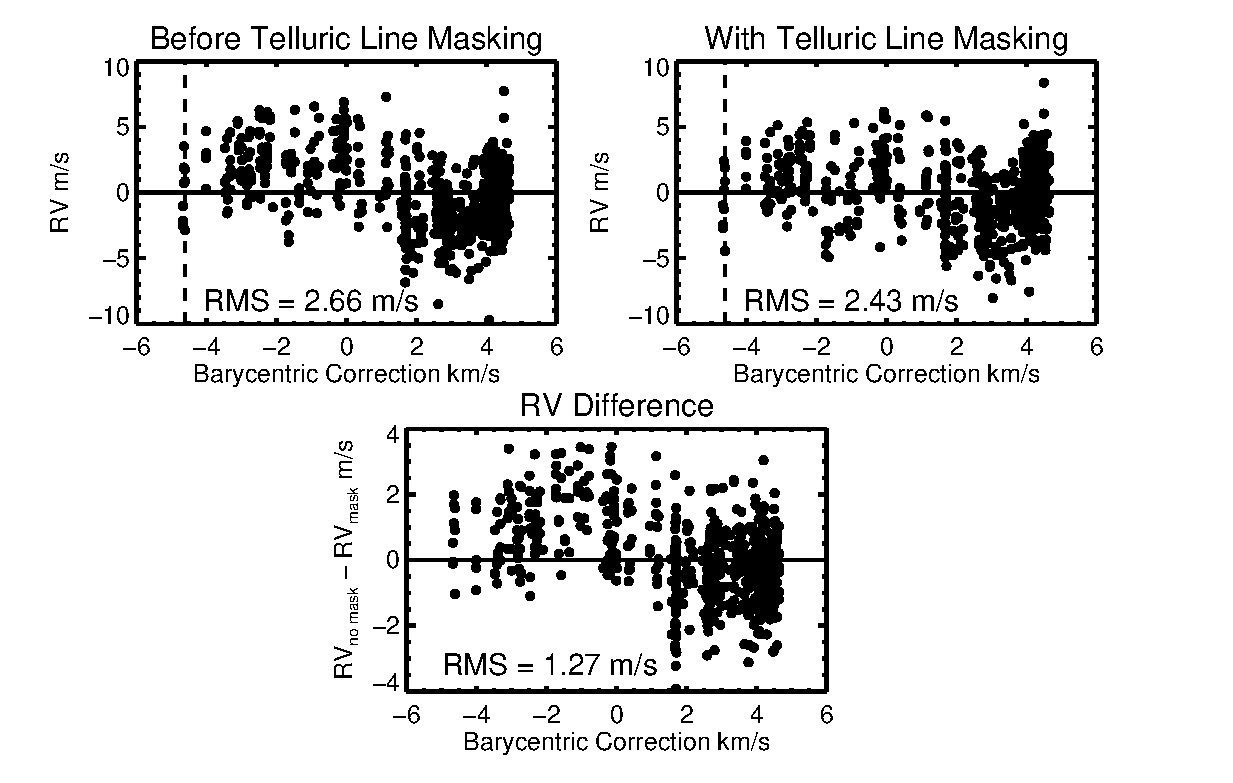
\includegraphics[width=0.48\textwidth]{telluric}
  \end{center}
  \vspace{-25pt}  
  \caption{Before and after making telluric lines.}
  \vspace{-8pt}  
  \label{tell}
\end{wrapfigure}


 
%%%%%%%%%%%%%%%%%%%%%%%%%%%%%%%%%%%%%%%%%%%%%%%%%%%%%%%%%%%%%%%%%%%%%%%%%%%%%%%%%%%%%%%%%
\vspace{-3pt}
\section{Relevance to NASA's Objectives and Missions}

Broadly, our investigation addresses one of the science
objectives of NASA SMD, ``Discover the origin, structure, evolution
and destiny of the universe and search for Earth-like planets".

More specifically, this proposal is directly and closely relevant to
the Astrophysics Research Program, theme (iii) Exoplanet Exploration,
in the solicitation:
\begin{itemize}[leftmargin=1.5em]
  \vspace{-3pt}
\item ``to search for planets and planetary systems about
  nearby stars in our Galaxy": This is the direct science goal of our
  work. 
  \vspace{-3pt}
\item ``to determine the properties of those stars that harbor
  planetary systems": We will acquire high resolution spectra on
  planet host stars with \keck\ and \hrs\ for, e.g. the
  \kepler\ stars, as required by the RV technique. Improved RV
  precision will also help better understanding stellar activities and
  stellar RV jitter.
  \vspace{-3pt}
\item ``to determine the percentage of planets that are in or near the
  Habitable Zone of a wide variety of stars and to measure their
  orbits": Improved RV precision of \keck\ and \hrs\ will enable more
  detections of potentially rocky exoplanets in the Habitable Zone of
  their host stars --- through both \kepler\ follow-up programs and
  independent RV surveys. Project \minerva\ will find more Earths and
  super-Earths in or near the Habitable Zone of nearby stars.
  \vspace{-3pt}
\end{itemize}

Our work will also support current and future NASA missions and
enhance their scientific outcome: (1) {\bf the \textit{Kepler}
  mission}: \keck\ and \hrs\ will directly support \kepler\ through
follow-up programs, including candidate validation/confirmation,
planetary mass measurements, TTV follow-up, and outer planet
discovery. {\bf (2) TESS:} \keck, \hrs, and \minerva can all
contribute significantly in follow-up programs on TESS targets. {\bf
  (3) JWST:} Finding more lower mass exoplanets means more Earth- or
super-Earth-like exoplanets, which are the primary targets for JWST
for planetary atmosphere characterization.


%%%%%%%%%%%%%%%%%%%%%%%%%%%%%%%%%%%%%%%%%%%%%%%%%%%%%%%%%%%%%%%%%%%%%%%%%%%%%%%%%%%%%%%%%
\vspace{-3pt}
\section{Relation to PI's Other NASA Grants}

The PI of this proposal, Prof.~Jason Wright, has received NASA Keck
time to search for long-period planet and multiple planet systems.
The PI has also received NASA Keck time to follow up a
\kepler\ planetary system with a strong TTV signal (Co-I Eric
Ford). Both of these programs will of no doubt benefit from the
improved Keck RV precision, and the upgraded \hrs\ is expected to
follow up some if not all of the long-period planet systems and
\kepler\ TTV systems in the future.


%%%%%%%%%%%%%%%%%%%%%%%%%%%%%%%%%%%%%%%%%%%%%%%%%%%%%%%%%%%%%%%%%%%%%%%%%%%%%%%%%%%%%%%%%
%\newpage
%\addcontentsline{toc}{section}{References}
\vspace{-3pt}
\bibliographystyle{apj}	% (uses file "xxx.bst")
{\small % smaller fonts for references
\bibliography{references} }

\end{document}
